%\documentclass[PhD,two side]{srmuthesis}
%\documentclass[MS]{srmuthesis}
%\documentclass[MTech]{srmuthesis}
\documentclass[BTech]{srmuthesis}
\usepackage{times}
\usepackage{t1enc}
\usepackage{tikz}
\usepackage{subfigure}
\usepackage{pgfplots}
\usepackage{setspace} 
\usepackage{geometry}
\usepackage{graphicx}
\usepackage{epstopdf}
\usepackage{lscape}
\usepackage{fancyhdr}
\usepackage{natbib}
\usepackage{hyperref} % hyperlinks for references.
\usepackage{amsmath} % easier math formulae, align, subequations \ldots
\usepackage{amssymb}
\usepackage{wasysym}
\usepackage{titlesec}
\usepackage{textcomp}
\usepackage{pifont}
\usepackage{appendix} 
\usetikzlibrary{decorations.pathmorphing}
\usetikzlibrary{shapes,arrows,shadows,patterns}
\usepackage[printonlyused]{acronym}
%\usepackage{nomencl}
%\newcommand{\bigsize}{\fontsize{16pt}{20pt}\selectfont}
%\renewcommand\nomname{\centerline {NOTATION}}
%\makenomenclature
\setcounter{MaxMatrixCols}{20}
\captionsetup[figure]{labelfont=bf}
\begin{document}
%%%%%%%%%%%%%%%%%%%%%%%%%%%%%%%%%%%%%%%%%%%%%%%%%%%%%%%%%%%%%%%%%%%%%%
% Title page

\title{Quote Attribution Using Deep Neural Networks} % Enter The Project Title

\firstauthor{ SAYAN DAS }% Enter The Student name
\firstauthorregno{[Reg No: RA1411003010485]}
\secondauthor{ SHUBHAM AGRAWAL }% Enter The Student name
\secondauthorregno{[Reg No: RA1411003010458]}
\thirdauthor{} % If there is no third author, leave the space blank like \thirdauthor{}
\thirdauthorregno{}
\fourthauthor{}
\fourthauthorregno{}
\fifthauthor{}
\fifthauthorregno{}
\guide{Mrs.J.Prathipa} % Enter your guide's name
\designation{Professor} % Enter your guide's designation
\guidedepartment{Computer Sciene \& Engineering} % Enter the department name of your Guide 
\hod{Dr.B.Amutha} % Enter HOD's name
\department{Computer Sciene \& Engineering} % Enter your department name
\date{MAY 2017} % Enter month and year of submission
%\nocite{*}

\maketitle
%%%%%%%%%%%%%%%%%%%%%%%%%%%%%%%%%%%%%%%%%%%%%%%%%%%%%%%%%%%%%%%%%%%%%%
%\vspace*{3in}
%\begin{center}
%{\Huge Dedicated to my Parents}
%\end{center}
%%%%%%%%%%%%%%%%%%%%%%%%%%%%%%%%%%%%%%%%%%%%%%%%%%%%%%%%%%%%%%%%%%%%%%
% Certificate
\certificate

%\vspace*{0.5in}


\begin{singlespace}
\tableofcontents
\thispagestyle{empty}

\pagenumbering{arabic}


\end{singlespace}

%%%%%%%%%%%%%%%%%%%%%%%%%%%%%%%%%%%%%%%%%%%%%%%%%%%%%%%%%%%%%%%%%%%%%%
% Abstract

\abstract
\begin{doublespacing}
{Conversation is the fundamental means for human interaction. Having back and forth interaction helps to understand the way one thinks, thus having a mutual understanding. It’s the beauty of brain how after a prolonged observation of same person conversing it starts to infer patterns. These patterns can either be the repetition of words or unique grammatical structure.
Here in this project I will try to replicate the same model using Natural
Language Processing and Neural Networks. For this given a quote the model will try to interpret the speaker based purely on the language based approach, i.e. no visual and auditory data are provided. Model will try to interpret context by using clues like “he said …” and “she told …” to understand the gender of the speaker. This can be achieved by using Recurrent Neural Network (RNN) which stores the context upto extent in the form of weights. Evaluation can be done by applying the predictive model to TV series episode scripts.}
\end{doublespacing}

\pagebreak
%%%%%%%%%%%%%%%%%%%%%%%%%%%%%%%%%%%%%%%%%%%%%%%%%%%%%%%%%%%%%%%%%%%%%%
% Acknowledgements
\acknowledgements
I would like to express my deepest gratitude to my guide, Mrs.J.Prathipa
his valuable guidance, consistent encouragement, personal caring, timely help and providing me with an excellent atmosphere for doing research. All through the work, in spite of his busy schedule, he has extended cheerful and cordial support to me for completing this research work.\\



\begin{flushright}
{\bf Author}
\end{flushright}


\chapter{Introduction}

Conversation is a fundamental means for human interaction. Following the back-and-forth thread of a conversation, as an interactive participant, is essential for constructing mutual understanding, but beyond this core competence we are generally able to drop in on a discussion already underway and similarly grasp its flow. Furthermore, after prolonged observation of the same parties conversing, we start to infer mental models for the speakers and develop expectations for what each speaker is more likely to say. These speaker models transcend the audible aspects of spoken conversation, and are founded instead upon the underlying language. In this work we consider the task of quote attribution (alternately, speaker identification) in the context of dialogue extracted from literary novels and television or movie screenplays. That is, given a sequence of unlabeled dialogue text, the aim is to classify each line according to its speaker. Performing this task well requires both an understanding of the temporal flow and the semantic substance of the dialogue lines. RNN-based approaches to modeling language have recently achieved state of-the-art performance  particularly owing to their ability to capture context (or in the case of streaming dialogue, “history”) of arbitrary length. RNNs thus seem a natural choice for learning the likelihood of a quote belonging to the lexicon of a particular character, as well as how to modify that likelihood conditioned on the prior sequence of conversation. 

\section{Problem Statement}

We consider a corpus $C = {E_1, . . . , E_k}$ consisting of dialogue extracted from a set of television episodes (or chapters, in the case of a literary novel). Each episode $E_k = { E_k^1 , . . . , E_k^{N_k} }$ is a sequence of dialogue lines, and each line $W_{(k,l)}  = {w_{(k,l)}^1 , . . . , w_{(k,l)}^{M_{k,l}} }$ is a sequence of word tokens, possibly spanning multiple sentences. Each line ` (k) l is associated with a label s (k) l denoting its speaker. Given a corpus of training episodes from the same television show, we consider the dialogue-only quote attribution problem of assigning speaker labels to lines from a previously unseen episode E˜ stripped of speaker tags. We evaluate the performance of a prediction model using a weighted average cross-entropy loss; we weight the loss to improve classification accuracy for less common speakers. To be precise, given one-hot ground truth speaker label vectors y (l) and corresponding predicted probability vector $y^{(l)}$ , we wish to minimize 

\chapter{Data and Pre Processing}

The dataset for this work consists of all episode screenplays from seasons 1–5 of Futurama scraped from http://www.imsdb.com/, the Internet Movie Script Database (IMSDb) For the purposes of training and evaluation, each line is labeled by the episode number as well as its true speaker label. No immediate context beyond utterance ordering is taken from the screenplays or novel.

Custom scrapper has been made using Beatiful Soup to extract the data from the above url sequentially and store the raw data as text file. 

\section{Cleaning}

Data has been cleaned using by designing specific regular expressions which swaps itself with the given target character. Some of the methods has been listed below:

\begin{itemize}
\item removeSpecialChars(): Removes the special characters and replaces with single space
\item removeBrackets(): Removes the content present in brackets.
\item removeMulSpacing(): Removes multiple spaces and replaces with single space
\end{itemize}

All the text has been converted to lower case. We have used nltk.wordtokenise to tokenise the sentence.

\section{Code}

\begin{verbatim}
'''
 Preprocessing Class
 Clean and process the raw files into <sess>.cleaned.bin

 Methods:
    cleanFile(): for a given file name it cleans and process data
    cleanName(): process speaker names
    cleanDial(): clean and process the dialogue
    tokenizeQuote(): tokenize the quote by words
'''

import pickle, os, re
import nltk
from config import Config

class Preprocess:

    def cleanFile(self, fname):
        script = open(fname, 'r').read().split('\n')
        cleaned = []
        for i in xrange(len(script)):
            row = script[i].split("\t")
            row[1] = self.cleanName(row[1])
            row[2] = self.cleanDial(row[2])
            cleaned.append([row[1], self.tokenizeQuote(row[2])])

        pickle.dump(cleaned, open("./data/cleaned.bin", 'wb'))
        del cleaned, script
        print "[SUCCESS] Cleaned at ./data/cleaned.bin"

    def cleanName(self, name):
        return name.strip().lower()

    def cleanDial(self, d):
        if not isinstance(d, list):
            d = d.strip().lower()
            d = re.sub(r'(\.\.+)|"|:|;', ' ', d) # Remove Multiple Spaces & Special ch.
            d = re.sub(r'\s*\([^)]*\)', '', d) # Remove bracket and it's content
            d = re.sub(r'\s+', ' ', d) # Remove Multiple Spaces
            return d.strip()
        else:
            return d

    def tokenizeQuote(self, quote):
        if not isinstance(quote, list):
            return nltk.word_tokenize(quote)
        else:
            return quote

if __name__ == '__main__':
    Preprocess().cleanFile(Config().rawData)

\end{verbatim}

\chapter{Quote Vector}

Given a quote $q$ consists of $\{w_1, w_2, w_3 ... w_n\}$ word vectors and the number of words ($n$) in each quote varies. Each word vector $w_i$ can be represented by $\{f_1^i, f_2^i, f_3^i ... f_d^i\}$. here in this case the dimension of the quote is of $n \times d$, to reduce the dimension we have taken the summary of each quote and thus reducing the dimension to $d$. We deviced 2 ways by which we can return qute vectors.

\section{Simple Averaging}

Here in this mean is taken of features of the word emebeding present in the give quote vertically. Formulae computes the quote vector of the given set of word vectors from the given quote.

\begin{center}
	$$\overrightarrow{\rm q} = \frac{1}{n} \sum_{i=1}^{n} f_k^i , \forall k \in \{1,2,3 ... d\} $$
\end{center}

\section{Sentence Level Embeding}

The proposed LSTM-RNN model sequentially takes each word in a sentence, extracts its information, and embeds it into a semantic vector. Due to its ability to capture long term memory, the LSTM-RNN accumulates increasingly richer information as it goes through the sentence, and when it reaches the last word, the hidden layer of the network provides a semantic representation of the whole sentence.

Although RNN performs the transformation from the sentence to a vector in a principled manner, it is generally difficult to learn the long term dependency within the sequence due to vanishing gradients problem. One of the effective solutions for this problem in RNNs is using memory cells instead of neurons originally proposed in as Long Short-Term Memory (LSTM) and completed in and by adding forget gate and peephole connections to the architecture.



\chapter{n-Way Multi Layer Neural Network Model}

This model consist of 3 layered neural network. With first layer consist of input layer and the third layer as the output layer. Input layer is same as the dimension of the quote vector and the output layer as the number of speakers. Here 'n' states the number of speakers as the output. As the number of speakers in the dataset is more than the dimensions hence we have reduced the number of speakers to 5. Number of speakers are chosen on the basis of hom much he/she speaks and the importance of the speaker on the plot. Number of hidden layers are manually auto tuned to get better F-measure scores. 


\tikzset{%
  every neuron/.style={
    circle,
    draw,
    minimum size=1cm
  },
  neuron missing/.style={
    draw=none, 
    scale=4,
    text height=0.333cm,
    execute at begin node=\color{black}$\vdots$
  },
}

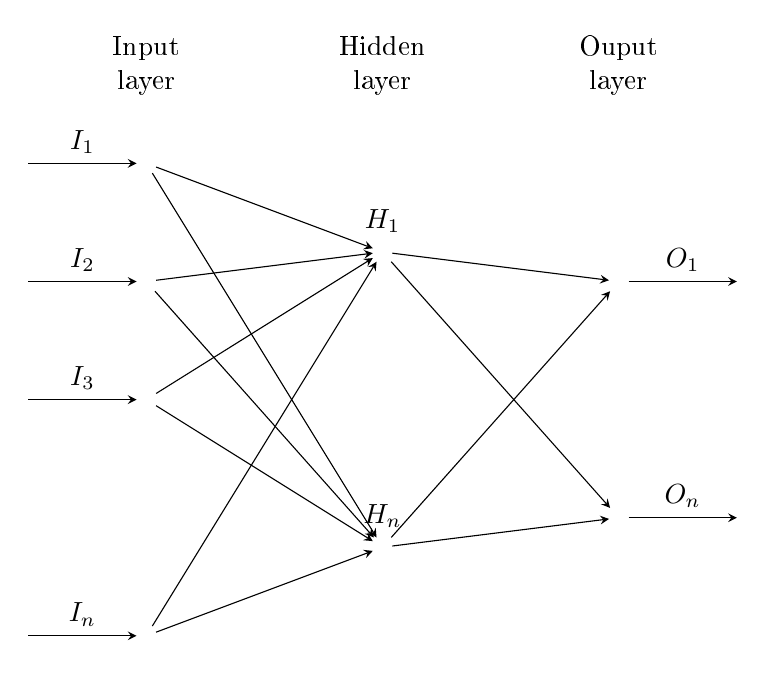
\begin{tikzpicture}[x=1.5cm, y=1.5cm, >=stealth]

\foreach \m/\l [count=\y] in {1,2,3,missing,4}
  \node [every neuron/.try, neuron \m/.try] (input-\m) at (0,2.5-\y) {};

\foreach \m [count=\y] in {1,missing,2}
  \node [every neuron/.try, neuron \m/.try ] (hidden-\m) at (2,2-\y*1.25) {};

\foreach \m [count=\y] in {1,missing,2}
  \node [every neuron/.try, neuron \m/.try ] (output-\m) at (4,1.5-\y) {};

\foreach \l [count=\i] in {1,2,3,n}
  \draw [<-] (input-\i) -- ++(-1,0)
    node [above, midway] {$I_\l$};

\foreach \l [count=\i] in {1,n}
  \node [above] at (hidden-\i.north) {$H_\l$};

\foreach \l [count=\i] in {1,n}
  \draw [->] (output-\i) -- ++(1,0)
    node [above, midway] {$O_\l$};

\foreach \i in {1,...,4}
  \foreach \j in {1,...,2}
    \draw [->] (input-\i) -- (hidden-\j);

\foreach \i in {1,...,2}
  \foreach \j in {1,...,2}
    \draw [->] (hidden-\i) -- (output-\j);

\foreach \l [count=\x from 0] in {Input, Hidden, Ouput}
  \node [align=center, above] at (\x*2,2) {\l \\ layer};

\end{tikzpicture}

\section{Feed Forward Method}

Feed forward network is used to predict the speaker. In this the information is passed from left to right using the following:

\begin{center}
	$f(\overrightarrow{\rm q}) = W.\overrightarrow{\rm q} + b$\\
	$h = sigmoid(f(\overrightarrow{\rm q}))$\\
	$\hat{y} = softmax(h)$
\end{center}

The activation functions of the hidden layer and the out put layer has been carefully chosen to obtain the best performance possible. Here in this case due to the limitation of the hardware specification we used Simple Averaging method to obtain the input quote vector.

\section{Training}

Training has been done using delta rule. Taking the loss function as the entropy loss function with adam's optimiser. Backpropagation is the key algorithm that makes training deep models computationally tractable. For modern neural networks, it can make training with gradient descent as much as ten million times faster, relative to a naive implementation. Thats the difference between a model taking a week to train and taking 200,000 years.

\begin{center}
$C= -\frac{1}{n} \sum x [y \ln a+(1−y)\ln(1−a)]$
\end{center}

Derivation for error propagation from the output layer to the hidden layer.

\begin{center}
$g'_{tanh}(z) = \frac{\partial}{\partial z} \frac{\text{sinh}(z)}{cosh(z)}$ \\  
$= \frac{\frac{\partial}{\partial z} \text{sinh}(z) \times \text{cosh}(z) - \frac{\partial}{\partial z} \text{cosh}(z) \times \text{sinh}(z)}{\text{cosh}^2(z)}$ \\ 
$= \frac{cosh^2(z) - sinh^2(z)}{cosh^2(z)}$ \\  
$= 1 - \frac{sinh^2(z)}{cosh^2(z)}$ \\  
$= 1 - \tanh^2(z)$
\end{center}

\section{Model Performance}

Model has been trained for 1000 epochs, with learning rate of 0.2. Hidden layer consist of 220 nodes. Training time to train 70\% of dataset was 26minutes.


Below contains the confuson matrix for 7 speakers, namely "fry", "bender", "leela", "farnsworth", "zoidberg", "amy" and others. 
$$\begin{pmatrix}
279&193&73&2&0&2&299\\
148&171&29&0&0&0&208\\
183&117&78&1&1&1&282\\
44&43&24&2&0&0&171\\
43&59&9&0 &1&1&94\\
49&37&10&0& 0&64\\
320&310&138&8&1&2&1020
\end{pmatrix}$$

F-measures for the same 7 speakers are as follows
$$\begin{pmatrix}
0.29153605&0.23014805&0.15234375 &0.01342282&0.00952381&0.&0.51816104
\end{pmatrix}$$


\section{Code}

\begin{verbatim}
'''
 Multi Layered Perceptron Model
 3 layered perceptron model with
 1st Layer[Input Layer]: 50 nodes [config.wordDim]
 2nd Layer[Hidden Layer]: 1200 Nodes [config.mlp['nHidden']]
 3rd Layer[Output Layer]: 65 Nodes [util.nSpeakers]

 H = sigmoid(X.W1)
 Yhat = softmax(H.W2)

 Test Accuracy: 36.96%
 Train Accuracy: 41.98%
'''



import tensorflow as tf
import numpy as np
import os, pickle, sys
sys.path.insert(0,'..')
from config import Config
from util import Util
import test

class mlp:
    def __init__(self):
        self.config = Config()
        self.util = Util()
        self.name = "MLP Model"

        X, Y = self.util.loadData(redChars=True)
        trainLen = int(X.shape[0]*self.config.mlp['train'])
        self.Xtrain, self.Xtest = X[:trainLen], X[trainLen:]
        self.Ytrain, self.Ytest = Y[:trainLen], Y[trainLen:]

    def forwardProp(self, X, W1, W2):
        h = tf.nn.sigmoid(tf.matmul(X, W1))
        yhat = tf.matmul(h, W2)
        return yhat

    def initWeight(self, shape):
        weight = tf.random_normal(shape, stddev=self.config.mlp['stddev'])
        return tf.Variable(weight)

    def model(self):
        self.X = tf.placeholder("float", shape=(None, self.config.wordDim))
        self.y = tf.placeholder("float", shape=(None, self.util.nSpeakers))

        self.W1 = self.initWeight([self.config.wordDim, self.config.mlp['nHidden']])
        self.W2 = self.initWeight([self.config.mlp['nHidden'], self.util.nSpeakers])

        self.yhat = self.forwardProp(self.X, self.W1, self.W2)
        self.predict = tf.argmax(self.yhat, axis=1)

        self.cost = tf.reduce_mean(tf.nn.softmax_cross_entropy_with_logits(labels=self.y, logits=self.yhat))
        self.update = tf.train.GradientDescentOptimizer(self.config.mlp['alpha']).minimize(self.cost)

    def train(self):
        print "Xtrain:", self.Xtrain.shape, "Xtest:", self.Xtest.shape
        print "Ytrain:", self.Ytrain.shape, "Ytest:", self.Ytest.shape

        sess = tf.Session()
        init = tf.global_variables_initializer()
        sess.run(init)

        saver = tf.train.Saver()
        for epoch in xrange(self.config.mlp['epochs']):
            sess.run(self.update, feed_dict={
                self.X: self.Xtrain,
                self.y: self.Ytrain
            })

            trainAccuracy = np.mean(np.argmax(self.Ytrain, axis=1) ==
                                 sess.run(self.predict, feed_dict={
                                 self.X: self.Xtrain,
                                }))
            testAccuracy  = np.mean(np.argmax(self.Ytest, axis=1) ==
                                 sess.run(self.predict, feed_dict={
                                 self.X: self.Xtest,
                                }))
            if epoch%self.config.mlp['disp'] == 0:
                print "Epoch = %d, train accuracy = %.2f%%, test accuracy = %.2f%%" % (epoch + 1, 100. * trainAccuracy, 100. * testAccuracy)

        save_path = saver.save(sess, self.config.mlp['modelPath'])
        print "Model saved in file: %s" % save_path
        sess.close()

    def forecast(self, X):
        saver = tf.train.Saver()
        with tf.Session() as sess:
            saver.restore(sess, self.config.mlp['modelPath'])
            Yhat = sess.run(self.predict, feed_dict={
                self.X: X
            })
            return Yhat

if __name__ == '__main__':
    os.chdir('..')

    obj = mlp()
    obj.model()
    # obj.train()
    test.genReport(obj.Ytest, obj.forecast(obj.Xtest))

\end{verbatim}

\chapter{Single Layered LSTM-Recurrent Neural Network Model}

When humam try to understand text, we do not every time start thinking from scratch. As we read essay we understand each and every word based on our understanding ofprevious words.We don't throw everything and start reading from the scratch. Our thought have persistance. 
We tried to replicate this same phenomenon in this model. As the traditional neural network does not do this. If we chain the neuraon passing messages from one node to another. This chain-like structure nature reveals that recurrent neural networks are initimately related to sequences and list.  

\begin{figure}[h]
\includegraphics[scale=0.4]{RNN-unrolled.png}
\centering
\end{figure}

\section{Drawbacks with normal Recurrent Neural Network}

One of the appeals of RNNs is the idea that they might be able to connect previous to the presetn task. Sometimes, we only need to look at recent information to perform the present task. But there also cases we need more context. Consider trying to predict the last word in the text “I grew up in France… I speak fluent French” Recent information suggests that the next word is probably the name of a language, but if we want to narrow down which language, we need the context of France, from further back. It’s entirely possible for the gap between the relevant information and the point where it is needed to become very large.

\section{LSTM Networks}

Long Short Term Memory networks – usually just called “LSTMs” – are a special kind of RNN, capable of learning long-term dependencies. They were introduced by Hochreiter and Schmidhuber (1997), and were refined and popularized by many people in following work. They work tremendously well on a large variety of problems, and are now widely used.

LSTMs are explicitly designed to avoid the long-term dependency problem. Remembering information for long periods of time is practically their default behavior, not something they struggle to learn!

All recurrent neural networks have the form of a chain of repeating modules of neural network. In standard RNNs, this repeating module will have a very simple structure, such as a single tanh layer.


\begin{figure}[h]
\includegraphics[scale=0.4]{LSTM3-chain.png}
\centering
\end{figure}

The key to LSTMs is the cell state, the horizontal line running through the top of the diagram.
The cell state is kind of like a conveyor belt. It runs straight down the entire chain, with only some minor linear interactions. It’s very easy for information to just flow along it unchanged. The LSTM does have the ability to remove or add information to the cell state, carefully regulated by structures called gates.

Gates are a way to optionally let information through. They are composed out of a sigmoid neural net layer and a pointwise multiplication operation.

The sigmoid layer outputs numbers between zero and one, describing how much of each component should be let through. A value of zero means “let nothing through,” while a value of one means “let everything through!”

An LSTM has three of these gates, to protect and control the cell state.

\section{Model Performance}

Model has been trained for 1000 epochs, with learning rate of 0.2. Number of states for each batch are 4 with each of size 22. Training time to train 70\% of dataset was 26minutes.


Below contains the confuson matrix for 7 speakers, namely "fry", "bender", "leela", "farnsworth", "zoidberg", "amy" and others. 
$$\begin{pmatrix}
67&3&42&0&0&0&736\\
42&8 &8&0&0&0&498\\
37&3&29&0&0&0&594\\
9&5&12&0&0&0&257\\
12&3&6&0&0&0&186\\
6&6&8&0&0&0&141\\
7&12&54&0&0&0&1660\\
\end{pmatrix}$$

F-measures for the same 7 speakers are as follows
$$\begin{pmatrix}
0.1228231&0.0268456&0.0705596&0.&0.&0.&0.56558773
\end{pmatrix}$$

\section{Code}

\begin{verbatim}
'''
 Recurrent Neural Network Model
 3 layered RNN Models with defferent cell types
 with L2 Regularization using Dropout optimization

 Input Dimension Def.: Batch Size X Num Steps X Input Vector
 Output Dimension Def.: Batch Size * Num Steps X Speaker Vector
'''

import tensorflow as tf
import numpy as np
import os, pickle, sys
sys.path.insert(0, '..')

from config import Config
from util import Util
import sklearn.metrics as metrics
import test


class rnn:
    def __init__(self, cellType="basic", wrapDropout=False, redChars=False):
        self.cellType = cellType
        self.wrapDropout = wrapDropout
        self.name = self.cellType + " Cell Type RNN Model"

        self.config = Config()
        self.config.rnn = self.config.rnn[self.cellType]
        self.util = Util()

        X, Y = self.util.loadData(redChars=redChars)
        trainLen = int(X.shape[0]*self.config.rnn['train'])
        self.Xtrain, self.Xtest = X[:trainLen], X[trainLen:]
        self.Ytrain, self.Ytest = Y[:trainLen], Y[trainLen:]

        self.Xtrain, self.Xtest = self.genBatch(self.Xtrain), self.genBatch(self.Xtest)
        self.Ytrain, self.Ytest = self.genBatch(self.Ytrain), self.genBatch(self.Ytest)

    def rnnCell(self):
        cell = None
        if self.cellType is "LSTM":
            cell = tf.contrib.rnn.LSTMCell(self.config.rnn['stateSize'])
            print "Loaded basic LSTM Cell"
        elif self.cellType is "basic":
            cell = tf.contrib.rnn.BasicRNNCell(self.config.rnn['stateSize'])
            print "Loaded basic RNN Cell"
        elif self.cellType is "GRU":
            cell = tf.contrib.rnn.GRUCell(self.config.rnn['stateSize'])
            print "Loaded GRU Cell"

        if self.wrapDropout:
            cell = tf.contrib.rnn.core_rnn_cell.DropoutWrapper(cell)
            print "Added Dropout Wrapper"
        # cell = tf.contrib.rnn.MultiRNNCell([cell]*2)
        return cell

    def genBatch(self, x):
        numStep = self.config.rnn['numStep']

        batchSize = x.shape[0] // numStep
        x = x[:batchSize*numStep-x.shape[0],:]
        x = x.reshape(batchSize, numStep, x.shape[-1])

        return x

    def model(self):
        self.X = tf.placeholder("float", shape=(None, self.config.rnn['numStep'], self.config.wordDim))
        self.y = tf.placeholder("float", shape=(None, self.config.rnn['numStep'], self.util.nSpeakers))

        cell = self.rnnCell()
        rnnOutputs, rnnStates = tf.nn.dynamic_rnn(cell, self.X, dtype="float")
        W = tf.Variable(tf.random_normal(shape=(self.config.rnn['stateSize'], self.util.nSpeakers), stddev=self.config.rnn['stddev']))
        b = tf.Variable(tf.constant(0.1, shape=[self.util.nSpeakers]))

        rnnOutputs = tf.unstack(rnnOutputs, num=self.config.rnn['numStep'], axis=1)

        logits = [tf.matmul(x, W)+b for x in rnnOutputs]
        logits = tf.stack(logits, axis=1)

        self.cost = tf.reduce_mean(tf.nn.softmax_cross_entropy_with_logits(labels=self.y, logits=logits))
        self.update = tf.train.AdamOptimizer(self.config.rnn['alpha']).minimize(self.cost)

        self.predict = tf.argmax(tf.reshape(logits, [-1, self.util.nSpeakers]),1)
        y_ = tf.argmax(tf.reshape(self.y, [-1, self.util.nSpeakers]),1)
        self.accuracy = tf.equal(self.predict, y_)

    def train(self):
        print "Xtrain:", self.Xtrain.shape, "Xtest:", self.Xtest.shape
        print "Ytrain:", self.Ytrain.shape, "Ytest:", self.Ytest.shape

        sess = tf.Session()
        init = tf.global_variables_initializer()
        sess.run(init)

        saver = tf.train.Saver()
        for epoch in xrange(self.config.rnn['epochs']):
            sess.run(self.update, feed_dict={
                self.X: self.Xtrain,
                self.y: self.Ytrain
            })

            trainAccuracy = np.mean(sess.run(self.accuracy, feed_dict={
                self.X: self.Xtrain,
                self.y: self.Ytrain
            }))

            testAccuracy = np.mean(sess.run(self.accuracy, feed_dict={
                self.X: self.Xtest,
                self.y: self.Ytest
            }))

            if (epoch+1) % self.config.rnn['disp'] == 0:
                print "Epoch = %d, train accuracy = %.2f%%, test accuracy = %.2f%%" % (epoch + 1, 100. * trainAccuracy, 100. * testAccuracy)

        save_path = saver.save(sess, self.config.rnn['modelPath'])
        print "Model saved in file: %s" % save_path
        sess.close()

    def forecast(self, X):
        saver = tf.train.Saver()
        with tf.Session() as sess:
            saver.restore(sess, self.config.rnn['modelPath'])
            Yhat = sess.run(self.predict, feed_dict={
                self.X: X
            })
            return Yhat

if __name__ == '__main__':
    os.chdir('..')

    obj = rnn(cellType="LSTM", redChars=True, wrapDropout=True)
    obj.model()
    # obj.train()

    test.genReport(obj.Ytest, obj.forecast(obj.Xtest))

\end{verbatim}


\chapter{Deep RNN Network with Contextual Sentence Embedder}

In the above models we have considered simple averaging technique for calculating the Quote Vector. Here in this method, high extent loss of criticaly important features.  So this method of calculating quote vector fundamentally wrong, in order to embed quote to vector. 

\section{Model Description}

This model can be divided into 4 layers. Each layer learn the each critically features which help to identify the speaker. 

1st layer is the input layer. This layer consist of single LSTM-RNN network and each network serve single node present in the next layer. Hence,  we can say that the input layer consist of 3 more layers. Due to the ability of the LSTM cell to capture the long term memory, the LSTM-RNN accumulates increasingly richer informationas it goesthrough the sentence, and when it reaches the last word, the hidden layer of the network provides a semantic representation of the whole sentence.

2nd layer is series of LSTM cells which captures the context of the speaker above the current speaker. LSTM cells helps to capture only the important features and forget the useless informations. Only the essential informations are passed from one node to another. And the same information is also passed to the upper layer also. 

3rd layer consist of GRU cells linked in a chain structure. This layer tries classify the user on the basis of the certain charecterstics which define the speaker. For example, if one character always uses the word 'Hey' at the begining of the statement then it's the responsibilty of this layer to capture this feature and classify the speaker.

\section{Model Performance}

Model has been trained for 1000 epochs, with learning rate of 0.2. State size for the 1st layer LSTM-RNN networks is considered as 10. 2nd layer LSTM cell chains have the state size of 50. 3rd layer the GRU cell chains have the size of 20. Training time to train 70\% of dataset was 47minutes.


Below contains the confuson matrix for 7 speakers, namely "fry", "bender", "leela", "farnsworth", "zoidberg", "amy" and others. 
$$\begin{pmatrix}
350&69&44&2&0&2&299\\
148&171&29&0&0&0&208\\
88&117&87&1&1&1&282\\
44&43&24&2&0&0&171\\
43&59&9&0 &1&1&94\\
49&37&10&0& 0&64\\
320&310&138&8&1&2&1020
\end{pmatrix}$$

F-measures for the same 7 speakers are as follows
$$\begin{pmatrix}
0.344&0.227&0.300&0.172&0.115&0.112&0.043&0.505
\end{pmatrix}$$


\section{Code}

\begin{verbatim}
'''
 Contextual Recurrent Neural Model
 [[ 170   76   38    0    3    0  560]
 [  65   66   16    1    0    0  408]
 [ 109   42   69    0    4    0  439]
 [  28   13   11    0    1    0  230]
 [  24   18    7    0    0    0  158]
 [  15   22   14    0    1    0  109]
 [ 150  121   69    4    4    1 1449]]
 [ 0.24147727  0.14442013  0.15558061  0.          0.          0.          0.5626092 ]
'''

import tensorflow as tf
import numpy as np
import os, pickle, sys
sys.path.insert(0, '..')

from config import Config
from util import Util
import test

class contRNN:
    def __init__(self):
        self.config = Config()
        self.util = Util()

        X, Y = self.util.loadData(redChars=True)
        trainLen = int(X.shape[0]*self.config.contRNN['train'])
        self.Xtrain, self.Xtest = X[:trainLen], X[trainLen:]
        self.Ytrain, self.Ytest = Y[:trainLen], Y[trainLen:]

        self.Xtrain, self.Xtest = self.genBatch(self.Xtrain), self.genBatch(self.Xtest)
        self.Ytrain, self.Ytest = self.genBatch(self.Ytrain), self.genBatch(self.Ytest)

    def genBatch(self, x):
        numStep = self.config.contRNN['numStep']

        batchSize = x.shape[0] // numStep
        x = x[:batchSize*numStep-x.shape[0],:]
        x = x.reshape(batchSize, numStep, x.shape[-1])

        return x

    def model(self):
        self.X = tf.placeholder('float', shape=(None, self.config.contRNN['numStep'], self.config.wordDim))
        self.y = tf.placeholder('float', shape=(None, self.config.contRNN['numStep'], self.util.nSpeakers))


        contOutput = self.addContextLayer()
        cell = tf.contrib.rnn.GRUCell(self.config.contRNN['stateSize'])
        cell = tf.contrib.rnn.core_rnn_cell.DropoutWrapper(cell)
        outputs, states = tf.nn.dynamic_rnn(cell, contOutput,  dtype='float')

        W = tf.Variable(tf.random_normal(shape=(self.config.contRNN['stateSize'], self.util.nSpeakers), stddev=self.config.contRNN['stddev']))
        b = tf.Variable(tf.constant(0.1, shape=[self.util.nSpeakers]))

        outputs = tf.unstack(outputs, num=self.config.contRNN['numStep'], axis=1)

        logits = [tf.matmul(x, W)+b for x in outputs]
        logits = tf.stack(logits, axis=1)

        self.cost = tf.reduce_mean(tf.nn.softmax_cross_entropy_with_logits(labels=self.y, logits=logits))
        self.update = tf.train.AdamOptimizer(self.config.contRNN['alpha']).minimize(self.cost)

        self.predict = tf.argmax(tf.reshape(logits, [-1, self.util.nSpeakers]),1)
        y_ = tf.argmax(tf.reshape(self.y, [-1, self.util.nSpeakers]),1)
        self.accuracy = tf.equal(self.predict, y_)

    # def addContextLayer(self):
    #     W = tf.Variable(tf.random_normal(shape=(self.config.wordDim, self.config.wordDim), stddev=self.config.contRNN['stddev']))
    #     b = tf.Variable(tf.constant(0.1, shape=[self.config.wordDim]))
    #
    #     X_ = tf.unstack(self.X, num=self.config.contRNN['numStep'], axis=1)
    #
    #     logits = [tf.tanh(tf.matmul(x, W)+b) for x in X_]
    #     return tf.stack(logits, axis=1)

    def addContextLayer(self):
        cell = tf.contrib.rnn.LSTMCell(self.config.contRNN['contStateSize'])
        cell = tf.contrib.rnn.core_rnn_cell.DropoutWrapper(cell)
        outputs, states = tf.nn.dynamic_rnn(cell, self.X, dtype="float")
        return outputs

    def train(self):
        print "Xtrain:", self.Xtrain.shape, "Xtest:", self.Xtest.shape
        print "Ytrain:", self.Ytrain.shape, "Ytest:", self.Ytest.shape

        sess = tf.Session()
        init = tf.global_variables_initializer()
        sess.run(init)

        saver = tf.train.Saver()

        for epoch in xrange(self.config.contRNN['epochs']):
            sess.run(self.update, feed_dict={
                self.X: self.Xtrain,
                self.y: self.Ytrain,
            })

            trainAccuracy = np.mean(sess.run(self.accuracy, feed_dict={
                self.X: self.Xtrain,
                self.y: self.Ytrain
            }))

            testAccuracy = np.mean(sess.run(self.accuracy, feed_dict={
                self.X: self.Xtest,
                self.y: self.Ytest
            }))

            if (epoch+1) % self.config.contRNN['disp'] == 0:
                print "Epoch = %d, train accuracy = %.2f%%, test accuracy = %.2f%%" % (epoch + 1, 100. * trainAccuracy, 100. * testAccuracy)

        save_path = saver.save(sess, self.config.contRNN['modelPath'])
        print "Model saved in file: %s" % save_path
        sess.close()

    def forecast(self, X):
        saver = tf.train.Saver()
        with tf.Session() as sess:
            saver.restore(sess, self.config.contRNN['modelPath'])
            Yhat = sess.run(self.predict, feed_dict={
                self.X: X
            })
            return Yhat

if __name__ == '__main__':
    os.chdir('..')

    obj = contRNN()
    obj.model()
    obj.train()

    test.genReport(obj.Ytest, obj.forecast(obj.Xtest))

\end{verbatim}


\chapter{Conclusion}

We have shown that using n-Way Multi Layered Neural Networks for conversation following provides improved performance over simpler neural network models at the task of dialogue-only quote attribution for screenplays and novels. Yet there is clearly still much
room for improvement. Alternative methods of quote summarization, may provide more
accurate windows into speaker personality. Allowing for selective retraining of word vectors, in
particular for tokens corresponding to speaker names, may also lead to better performance. Figure 1
shows the GloVe word vectors for a selection of character tokens (plus a few additional words) plotted
by their components along the vectors’ first two principal axes. In the context of the Gigaword5
+ Wikipedia2014 corpus, all of the Futurama characters are essentially equivalent. For the purpose
of quote attribution, however, we’d like the word “bender” in the exchange from Table 1 to send a
strong signal that the next speaker is likely to be Bender. We expect that such word vector retraining
would increase the benefits provided by using a recursive neural network in Layer 2 (conversational
context).

  \end{document}
